\documentclass[margin=5mm]{standalone}
\usepackage[T1]{fontenc}
\usepackage[utf8]{inputenc}
\usepackage{pgf,tikz}
\usepackage{utfsym}

\newcommand{\wheel}{%
  \draw[fill, black!60] (-3mm, -1mm) rectangle (3mm, 1mm); }

\newcommand{\robot}{%
  \node[anchor=center,circle, draw, inner sep=5mm] at (0,0) {};
  \begin{scope}[xshift=-2mm, yshift=5mm]
    \wheel
  \end{scope}
  \begin{scope}[xshift=-2mm, yshift=-5mm]
    \wheel
  \end{scope}
  \node[anchor=center, circle, inner sep=1mm, black!60,fill] at (4mm, 0) {};
  \draw[->, red!60!black] (0,0) to (20mm, 0);
  %\node at (20mm, 4mm) {$v$};
  %\draw[->, red!60!black] (0, 2.7mm) arc[radius=2.7mm, start angle=90, end angle=270];
  %\node at (-4mm, 1mm) {$\omega$};
}

  \begin{document}

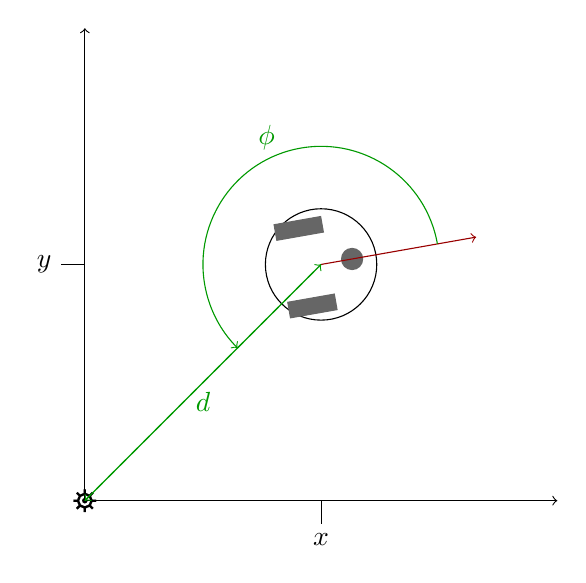
\begin{tikzpicture}[node distance=20mm, anchor=north]

  \draw[->] (0,0) to (6cm, 0);
  \draw[->] (0,0) to (0, 6cm);

  \node[anchor=center] at (0,0) {\large \usym{26EF}};

  \begin{scope}[xshift=3cm, yshift=3cm, rotate=10]
    \robot
  \end{scope}

  \draw[green!60!black, dashed]  (0,0) to (3, 3);
  \pgfmathsetmacro{\xp}{ 3 + 1.5*cos(10)}
  \pgfmathsetmacro{\yp}{ 3 + 1.5*sin(10)}
  \draw[green!60!black,->] (\xp, \yp) arc[radius=15mm, start angle=10, end angle=225] node[above, pos=0.5] {$\phi$};
  \draw[green!60!black, <->]  (0,0) to node[below] {$d$} (3, 3);
  
  \draw (3, 0) -- (3, -0.3) node[below] {$x$};
  \draw (0, 3) -- (-0.3, 3) node[left] {$y$};

  %\draw[dashed] (3, 3) to (5, 3); 

  
\end{tikzpicture}
\end{document}
